\phantomsection
\chapter{Viola-Jones}

\noindent Viola-Jones algorithm is "a visual object detection framework that is capable of processing images extremely rapidly while achieving high detection rates". 3 main points characterize this algorithm. The first one is the use of what is called an "Integral image". It is a new representation of the image and it allows the features used to be computed very quickly. The second one is the use of a learning algorithm based on AdaBoost. It results in giving extremely efficient classifiers. The third and last one is the use of a method to combine classifiers. This method combine classifiers in "cascade". It allows to focus on the promising object-like regions by discarding the background in a very quick way \cite{VIO01}.
\newline

\phantomsection
\section{Overview}

\vspace{\baselineskip}
\noindent The Viola-Jones algorithm works as following \cite{DIN08}:

\begin{itemize}
  \item "The Viola-Jones detector is a strong, binary classifier build of several weak detectors"
  \item "Each weak detector is a simple binary classifier"
  \item During the learning part, a cascade of weak classifiers is used and trained in order to attained the desired hit/miss rate using the learning algorithm based on AdaBoost
  \item The input image is divided in several rectangular sub-regions in order to detect objects. The cascade computes each of these sub-regions
  \item To classify a sub-region as "positive", it has to go through all of the stages of the cascade
  \item All the process involving the sub-regions is repeated at different scales
\end{itemize}

\phantomsection
\section{Haar features}

\vspace{\baselineskip}
\noindent The features used by Viola and Jones are called Haar features and are based on Haar wavelets. Haar wavelets are single wavelength square waves. It is composed of one high interval and one low interval. In two dimensions, a square wave is represented by a pair of adjacent rectangles: one rectangle that is light and one rectangle that is dark. The true Haar wavelets are not the one used for this rectangle combinations that is used for visual object detection. They use instead rectangle combinations that are better suited to recognition tasks. That is because of this difference that these features are called Haar features rather than Haar wavelets (they can also be called Haarlike features) \cite{HEW07}.
\newline

\noindent For example, the figure~\ref{haar_features_first_2_stage} shows the first two Haar features in the original Viola-Jones cascade \cite{HEW07}. These are all features from the original set of features. In figure~\ref{haar_features_extended}, there is an example of features from the extended set of features \cite{DIN08}. In the figure~\ref{haar_features_early_stage} , it is an example of a early stage in the Haar cascade. Each black and white rectangle represents a feature. And that is what the algorithm hunts for in the image \cite{HAR12}.
\newline

\begin{figure}[!h]
\begin{center}
\noindent 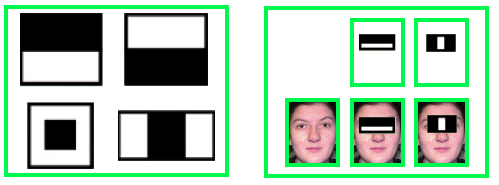
\includegraphics[scale=0.9]{figures/haar_features_first_2_stage} 
\newline
\caption{Example of the first two Haar features}
\label{haar_features_first_2_stage}
\end{center} 
\end{figure}

\begin{figure}[!h]
\begin{center}
\noindent 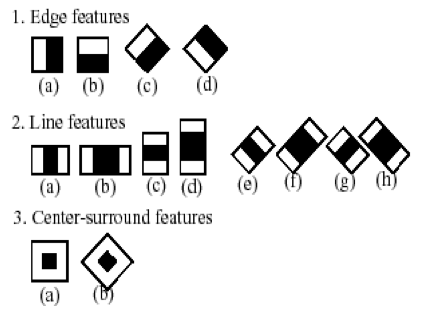
\includegraphics[scale=0.6]{figures/haar_features_extended} 
\newline
\caption{Extended set of features}
\label{haar_features_extended}
\end{center} 
\end{figure}

\begin{figure}[!h]
\begin{center}
\noindent 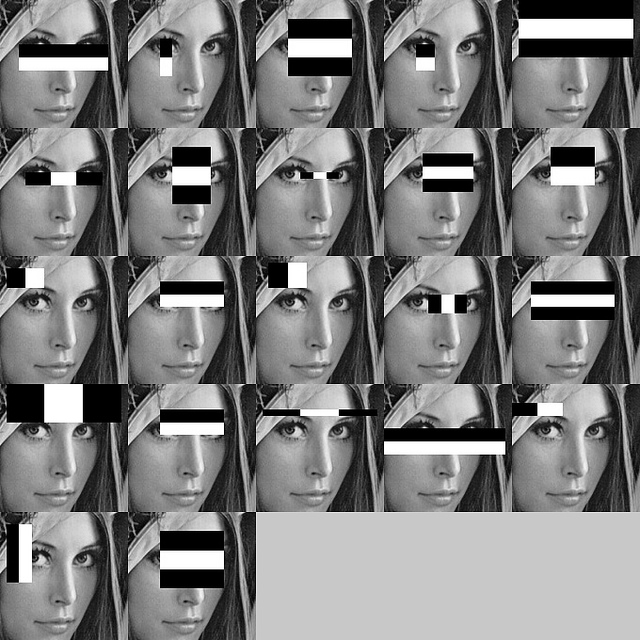
\includegraphics[scale=0.5]{figures/haar_features_early_stage} 
\newline
\caption{Example of an early stage in the Haar cascade}
\label{haar_features_early_stage}
\end{center} 
\end{figure}

\noindent To detect if a Haar feature is present or not, basic subtraction is used. The subtraction consists in subtracting the average pixel value of the dark-region from the average pixel value of the light-region. Then it is a simple comparison. The result of the subtraction is compared with a threshold. If the result is above the threshold, then the feature is considered as present and it can go to the next stage \cite{HEW07}. There is about 20 to 30 different stages to detect the presence of Haar features. The first stage is a very coarse scan of the image. The second stage is more detailed, the third stage is once again more detailed and harder to pass, the fourth stage is even harder and it goes on and on till the end. The more it moves froward into the cascade, the more it becomes harder. The features become increasingly complex and larger. All this processing takes indeed more time to compute \cite{HAR12}.
\newline

\noindent For example, the figure~\ref{haar_feature_later_stage} shows the later stage in the Haar cascade. There are many more patterns of black and white rectangles that need to match the input image \cite{HAR12}.
\newline

\begin{figure}[!h]
\begin{center}
\noindent 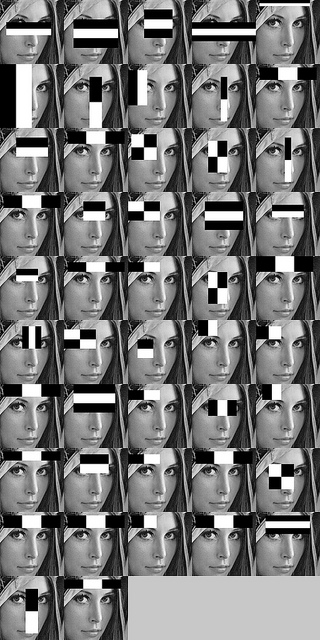
\includegraphics[scale=0.8]{figures/haar_feature_later_stage} 
\newline
\caption{Example of the later stage in the Haar cascade}
\label{haar_feature_later_stage}
\end{center} 
\end{figure}

\noindent It exists three kinds of feature that Viola and Jones use: a two-rectangle feature, a three-rectangle feature and a four-rectangle feature. To find the value of the two-rectangle feature, it consists in the difference between the sum of the pixels that are in the two rectangular regions. The regions (or rectangles) are the same: they have the same size and the same shape. And they are horizontally or vertically adjacent. The three-rectangle feature are calculated by the sum of the pixels of the two outside rectangles subtracted from the sum of the pixels in the center rectangle. The last kind of feature is the four-rectangle feature consists in the difference between the diagonal pairs of rectangles \cite{VIO01}.
\newline

\noindent For example, the figure~\ref{haar_feature_description} shows the different kinds of rectangle features used by the Viola-Jones algorithm. The images (A) and (B) show the two-rectangle features. The image (C) shows the three-rectangle feature, and the image (D) shows the four-rectangle feature \cite{VIO01}.
\newline

\begin{figure}[!h]
\begin{center}
\noindent 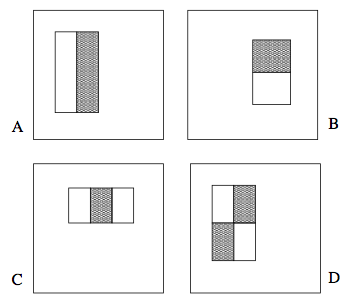
\includegraphics[scale=0.6]{figures/haar_feature_description} 
\newline
\caption{Example of the different kinds of rectangle features}
\label{haar_feature_description}
\end{center} 
\end{figure}

\noindent Viola and Jones admit that rectangle features can be considered as primitive features. In contrast with other features, rectangle features are quite coarse (even though they are sensitive to the presence of edges, bars and other simple image structure). It appears that however, a rich image representation is provided by this set of rectangle features and furthermore this representation supports effective learning. In comparison with the extreme computational efficiency provided by rectangle features, their limited flexibility is not much of a problem \cite{VIO01}.
\newline

\phantomsection
\section{Integral image}

\vspace{\baselineskip}
\noindent Viola and Jones used an intermediate representation of an image that they called "integral image". This integral image allows to compute very quickly the rectangle features \cite{VIO01}. This technique allows to determine the presence or absence of hundreds of Haar features. It can be determined for every image location and for several scales efficiently. In general, adding small units together is what is called "integrating"; here, the small units are pixel values. The sum of all the pixels above and to the left of each pixel is the the integral value. And this value can be found for each pixel. That is why this technique is efficient: the entire image can be integrated only with a few calculations per pixel. This integration starts at the top left corner and go through all the image to the right and down \cite{HEW07}.
\newline

\noindent It means that the integral image, at location $ x,y $ contains the sum of the pixels above and on the left of $ x,y $, $ x,y$ included: \[ ii(x,y) = \sum_{x' \leq x,y' \leq y} i(x',y') \] where $ ii(x,y) $ is the integral image and $ i(x,y) $ is the regional image. In the figure~\ref{integral_image_description}, the value of the integral image at point $ (x,y) $ is the sum of all the pixels above and on the left \cite{VIO01}. 
\newline
	
\begin{figure}[!h]
\begin{center}
\noindent 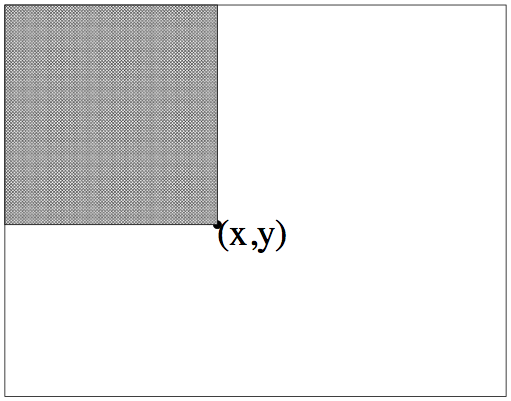
\includegraphics[scale=0.5]{figures/integral_image_description} 
\newline
\caption{Integral image}
\label{integral_image_description}
\end{center} 
\end{figure}
	
\noindent Using the following pair of recurrences: 
\begin{equation}
s(x,y) = s(x,y - 1) + i(x,y)
\end{equation}
\begin{equation}
ii(x,y) = ii(x - 1,y) + s(x,y)
\end{equation}
(where $ s(x,y) $ is the cumulative row sum, $ s(x,-1) = 0 $, and $ ii(-1,y) = 0 $) the integral image can be computed in one pass over the original image. 
\newline

\noindent Thanks to the integral image, any rectangular sum can be calculated in four array references. In the figure~\ref{integral_image_four_array}, the sum of the pixels in rectangle D can be calculated with four array references. The value of the integral image at the point 1 is the sum of the pixels in rectangle $ A $. The value at the point 2 is $ A + B $, at the point 3 is $ A + C $, and at the point 4 is $ A + B + C + D $. The sum in D can then be computed as $ 4 + 1 - (2 + 3) $ \cite{VIO01}. 
\newline

\begin{figure}[!h]
\begin{center}
\noindent 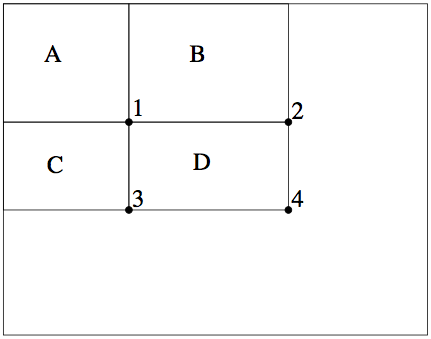
\includegraphics[scale=0.6]{figures/integral_image_four_array} 
\newline
\caption{Integral image with four array references}
\label{integral_image_four_array}
\end{center} 
\end{figure}

\phantomsection
\section{Weak classifiers and AdaBoost}

\vspace{\baselineskip}
\noindent Features are extracted from a sub-region of an input image. This sub-region has a size that is usually of 24 by 24 pixels. Each of all the features types are moved and scaled across the entire input image (In a 24 pixel by 24 pixel sub-region, it means that there are about 160,000 possible combinations to process) \cite{SMY07}.
\newline

\noindent AdaBoost is a machine-learning method used by Viola and Jones in order to select the specific Haar features to use. It is also used to set the threshold levels. This method is based on the combination of many weak classifiers to form a strong one. It is called a weak classifier because this kind of classifiers obtains the right answer only a little more often than a random guess would which is not particularly good. The purpose of using so many weak classifiers is to get a right answer with a higher rate of success. All of this is based on the verified hypothesis that if each of the weak classifiers pushes the final answer a little bit in the right direction each time, it means that at the end, the correct answer is obtained. This combination of several weak classifiers represents a strong one \cite{HEW07}. 
\newline

\noindent AdaBoost selects a set of weak classifiers to combine and assigns a weight to each (see figure~\ref{haar_feature_adaboost}). This weighted combination is the strong classifier \cite{HEW07}. The challenge is to associate a large weight with each good classification function and a smaller weight with poor functions. AdaBoost is an aggressive mechanism for selecting a small set of good classification functions which nevertheless have signficant variety \cite{VIO01}.
\newline

\begin{figure}[!h]
\begin{center}
\noindent 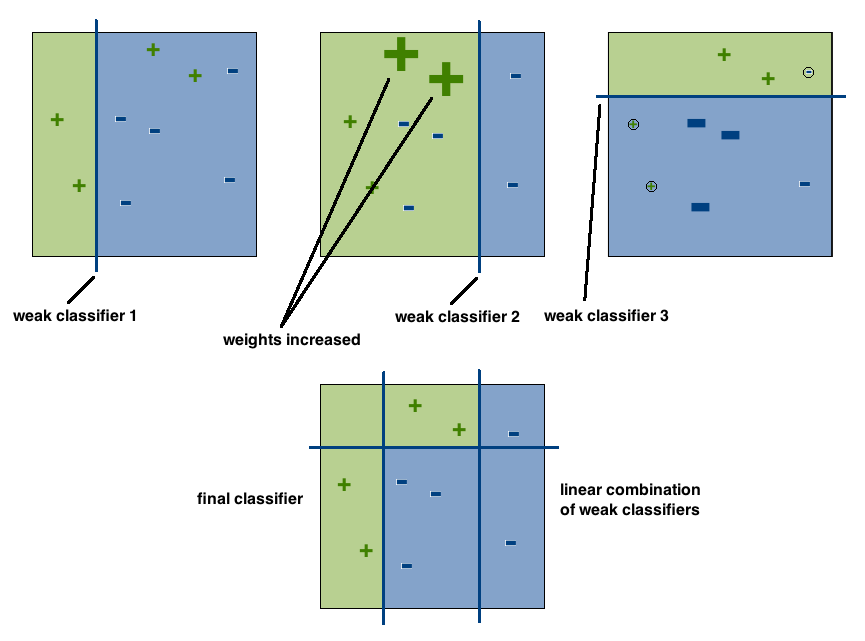
\includegraphics[scale=0.6]{figures/haar_feature_adaboost} 
\newline
\caption{AdaBoost method}
\label{haar_feature_adaboost}
\end{center} 
\end{figure}

\noindent Initial experiments demonstrated that a classifier constructed from 200 features using AdaBoost would yields reasonable results. Given a detection rate of 95\%, the classifier yielded a false positive rate of 1 in 14084 on a testing dataset (see figure~\ref{haar_feature_example_result})\cite{VIO01}.
\newline

\begin{figure}[!h]
\begin{center}
\noindent 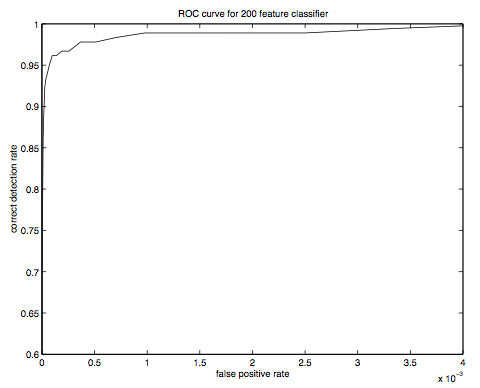
\includegraphics[scale=0.8]{figures/haar_feature_example_result} 
\newline
\caption{Receiver operating characteristic (ROC) curve for the 200 feature classifier}
\label{haar_feature_example_result}
\end{center} 
\end{figure}

\noindent The 200-feature classifier provides initial evidence that a boosted classifier constructed from rectangle features is an effective technique for object detection. In terms of detection, these results are compelling but not sufficient for many real-world tasks. In terms of computation, this classifier is probably faster than any other published system, requiring 0.7 seconds to scan an 384 by 288 pixel image. Unfortunately, the most straightforward technique for improving detection performance, adding features to the classifier, directly increases computation time \cite{VIO01}.
\newline

\phantomsection
\section{Classifiers cascade}

\vspace{\baselineskip}
\noindent Viola and Jones combined a series of AdaBoost classifiers as a filter chain, that is especially efficient for classifying image regions. Each filter is a separate AdaBoost classifier with fairly small number of weak classifiers. As in figure~\ref{haar_feature_cascade}, the classifier cascade is a chain of filters. Image subregions that make it through the entire cascade are classified as "Face". All others are classified as "Not Face" \cite{HEW07}. This algorithm for constructing a cascade of classifiers achieves increased detection performance while radically reducing computation time \cite{VIO01}.
\newline

\begin{figure}[!h]
\begin{center}
\noindent 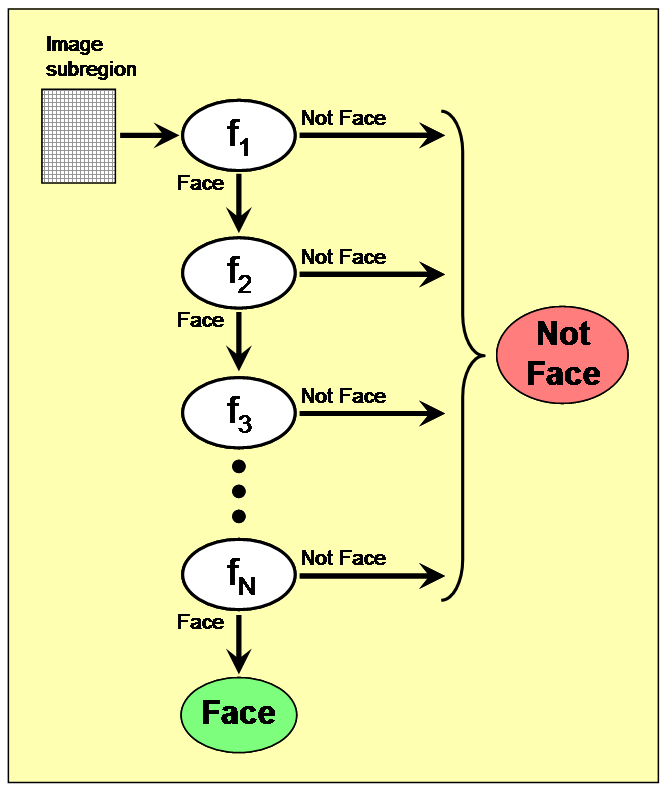
\includegraphics[scale=0.5]{figures/haar_feature_cascade} 
\newline
\caption{Cascade of boosted classifiers}
\label{haar_feature_cascade}
\end{center} 
\end{figure}

\noindent In order to explore the feasibility of the cascade approach two simple detectors were trained: a monolithic 200-feature classifier and a cascade of ten 20-feature classifiers. Figure~\ref{haar_feature_cascade_example_result} gives the ROC curves comparing the performance of the two classifiers. It shows that there is little difference between the two in terms of accuracy. However, there is a big difference in terms of speed. The cascaded classifier is nearly 10 times faster since its first stage throws out most non-faces so that they are never evaluated by subsequent stage \cite{VIO01}.
\newline

\begin{figure}[!h]
\begin{center}
\noindent 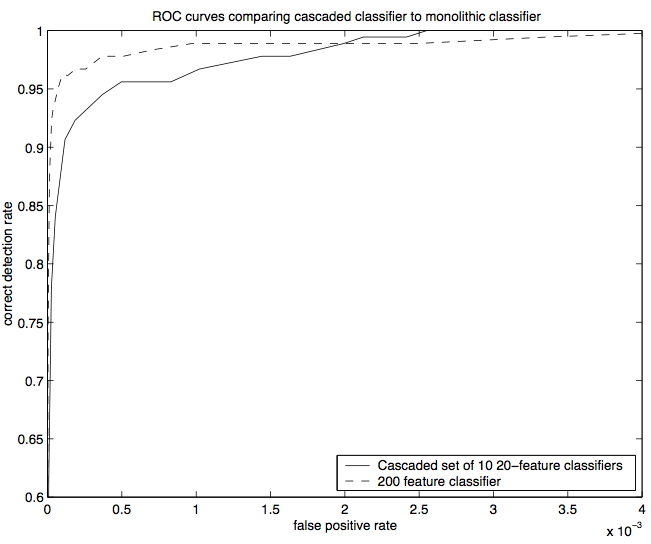
\includegraphics[scale=0.6]{figures/haar_feature_cascade_example_result} 
\newline
\caption{ROC curves comparing a 200-feature classifier with a cascaded classifier containing ten 20-feature classifiers}
\label{haar_feature_cascade_example_result}
\end{center} 
\end{figure}

\noindent The acceptance threshold at each level is set low enough to pass all, or nearly all, face examples in the training set. The filters at each level are trained to classifiy training images that passed all previous stages. During use, if anyone of these filters fails to pass an image region, that region is immediately classified as "Not Face". When a filter passes an image region, it goes to the next filter in the chain. Image regions that pass through all filters in the chain are classified as "Face". Viola and Jones named this filtering chain a cascade \cite{HEW07}.
\newline

\noindent The key insight is that smaller, and therefore more efficient, boosted classifiers can be constructed which reject many of the negative sub-windows while detecting almost all positive instances. Simpler classifiers are used to reject the majority of sub-windows before more complex classifiers are called upon to achieve low false positive rates \cite{VIO01}.
\newline

\noindent The order of filters in the cascade is based on the importance weighting that AdaBoost assigns. The more heavily weighted filters come first, to eliminate non-face image regions as quickly as possible. In figure~\ref{haar_feature_first_2_features}, it shows the first two features from the original Viola-Jones cascade superimposed on a face. The first one keys off the cheek area being lighter than the eye region. The second uses the fact that the bridge of the nose is lighter than the eyes \cite{HEW07}.
\newline

\begin{figure}[!h]
\begin{center}
\noindent 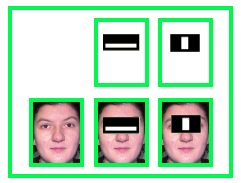
\includegraphics[scale=1]{figures/haar_feature_first_2_features} 
\newline
\caption{The first two Haar features in the original Viola-Jones cascade}
\label{haar_feature_first_2_features}
\end{center} 
\end{figure}

\noindent The structure of the cascade reflects the fact that within any single image an overwhelming majority of sub-windows are negative. As such, the cascade attempts to reject as many negatives as possible at the earliest stage possible. While a positive instance will trigger the evaluation of every classifier in the cascade, this is an exceedingly rare event \cite{VIO01}.
\newline

\noindent Following are the different numbers about cascade classifiers (see figure~\ref{haar_feature_cascade_rate}) \cite{UBC01}:

\begin{itemize}
  \item A 1 feature classifier achieves 100\% detection rate and about 50\% false positive rate
  \item A 5 feature classifier achieves 100\% detection rate and about 40\% false positive rate (20\% cumulative)
  \item A 20 feature classifier achieves 100\% detection rate and about 10\% false positive rate (2\% cumulative)
\end{itemize}

\begin{figure}[!h]
\begin{center}
\noindent 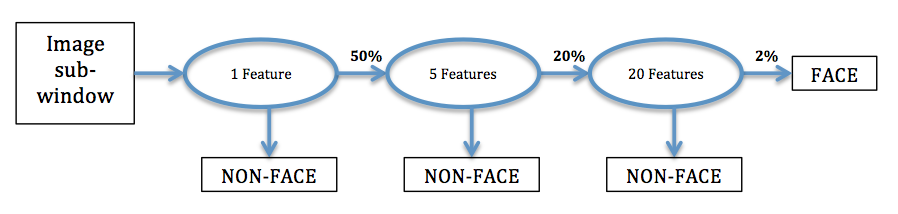
\includegraphics[scale=0.5]{figures/haar_feature_cascade_rate} 
\newline
\caption{Cascade of boosted classifiers rate}
\label{haar_feature_cascade_rate}
\end{center} 
\end{figure}

\phantomsection
\section{Test set and training}

\vspace{\baselineskip}
\noindent The face training set consisted of 4916 hand labeled faces scaled and aligned to a base resolution of 24 by 24 pixels. The faces were extracted from images downloaded during a random crawl of the world wide web. Some typical face examples are shown in figure~\ref{haar_feature_training_dataset} \cite{VIO01}.
\newline

\begin{figure}[!h]
\begin{center}
\noindent 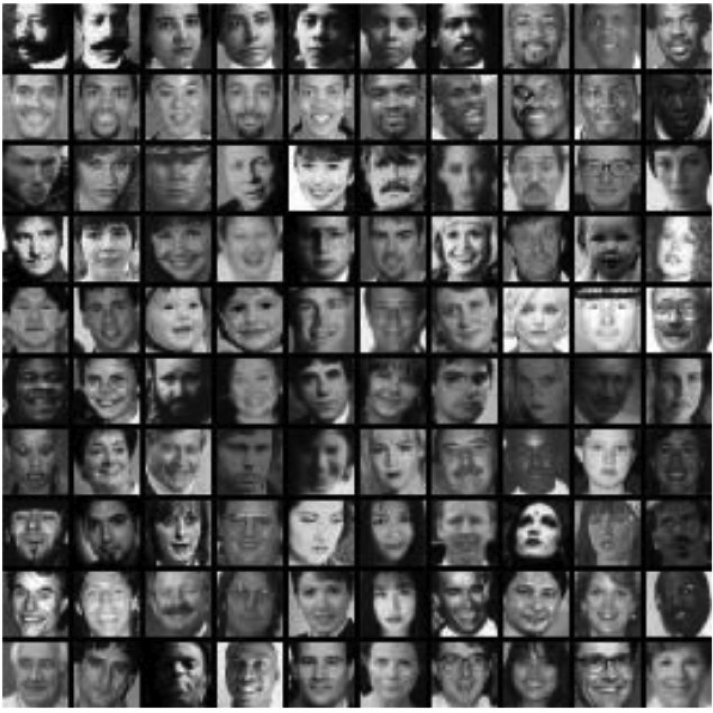
\includegraphics[scale=0.9]{figures/haar_feature_training_dataset} 
\newline
\caption{Example of frontal upright face images used for training}
\label{haar_feature_training_dataset}
\end{center} 
\end{figure}

\noindent The training set is composed of \cite{UBC01}:

\begin{itemize}
  \item 5,000 faces
  \begin{itemize}
  	\item All frontal
  \end{itemize}
  \item 300 million non faces
  \begin{itemize}
  	\item 9,400 non-face images
  \end{itemize}
  \item Face are normalized
  \begin{itemize}
  	\item Scale, translation
  \end{itemize}
  \item Many variations
  \begin{itemize}
  	\item Across individuals
	\item Lightning
	\item Pose (rotation both in plane and out)
  \end{itemize}
\end{itemize}

\vspace{\baselineskip}
\noindent The test set is usually divided into a training set and a validation set. A typical training set may contain about 5,000 positive samples (faces) and 10,000 negative samples (non-face sub-windows randomly chosen from non-face images) \cite{DIN08}. Training time for an entire 32 layer detector is on the order of weeks \cite{VIO01}.
\newline

\noindent Viola-Jones training stage proceeds with the following step \cite{DIN08}:

\begin{itemize}
  \item Given the number K of possible features (about 160,000 on a $ 24\times24 $ gray-level image)
  \item Fix the number L of desired stages in the cascade
  \item Iterate until L weak classifiers have been selected:
  \begin{itemize}
  	\item Given reweighed data from the previous stage
	\item Train all K weak classifiers (find the best threshold to classify the training set)
	\item Select the best classifier at this stage
	\item Reweight the data
  \end{itemize}
\end{itemize}

\noindent The weak classifiers are associated to weights thet depends on their classification error. Those weights are used in a linear combination of the weak classifiers which represents a huge computational cost \cite{DIN08}.
\newline





